%%%%%%%%%%%%%%%%%%%%%%%%%%%%%%%%%%%%%%%%%%%%%%%%%%%%%%%%%%%%%%%%%%%%%%%%%%%%%%%%%%%%%%%%%%%%%%%%%%%
%%%%%%%%%%%%%%%%%%%%%%%%%%%%%%%%%%%%%%%%%%%%%%%%%%%%%%%%%%%%%%%%%%%%%%%%%%%%%%%%%%%%%%%%%%%%%%%%%%%
%%%%%%%%%%%%%%%%%%%%%%%%%%%%%%%%%%%%%%%%%%%%%%%%%%%%%%%%%%%%%%%%%%%%%%%%%%%%%%%%%%%%%%%%%%%%%%%%%%%

\section{Aplicación de la prueba de Priestley-Subba Rao}

Se fragmentaron los registros en ventanas de 30 segundos de duración, sin traslape. Cada una de 
estas ventanas fue sometida a la prueba de PSR, y se clasificó como \textit{estacionaria en el 
sentido de PSR} si fue posible rechazar ($p<0.05$) la hipótesis de no-estacionariedad. 
%
Los resultados obtenidos (una lista de las épocas que son estacionarias) se guardaron en archivos 
de texto para su posterior análisis. 
%
Debido a la gran variabilidad entre el tiempo que los participantes pasaron en sueño MOR, se decidió
basar las comparaciones en proporciones de épocas; por ejemplo, se calculó la proporción de
épocas MOR que son estacionarias para todos los participantes.

%\begin{figure}
%\centering
%\begin{lstlisting}[caption={}]
%Priestley-Subba Rao stationarity Test for datos
%-----------------------------------------------
%Samples used              : 3072 
%Samples available         : 3069 
%Sampling interval         : 1 
%SDF estimator             : Multitaper 
%  Number of (sine) tapers : 5 
%  Centered                : TRUE 
%  Recentered              : FALSE 
%Number of blocks          : 11 
%Block size                : 279 
%Number of blocks          : 11 
%p-value for T             : 0.4130131 
%p-value for I+R           : 0.1787949 
%p-value for T+I+R         : 0.1801353 
%\end{lstlisting}
%\caption[Resultado típico para la función \texttt{stationarity}]
%{Resultado típico para la función \texttt{stationarity}. La función de densidad espectral es
%referida como SDF, mientras que los p valores. El p-valor para \texttt{T+I+R} corresponde al 
%estadístico $S_{I+R}$, y el p-valor para \texttt{T} corresponde $S_T$
%}
%\label{res_psr}
%\end{figure}

Como análisis exploratorio se graficaron en el tiempo las épocas, en todos los canales, como se 
muestra en la figura \ref{patroncito}. Este tipo de gráficos \textit{revelan} cierto tipo de 
\textit{bloques} de épocas estacionarias o no-estacionarias. Heurísticamente se puede afirmar que 
éstos patrones son independientes de la prueba de PSR, y anteriormente se reportó que estos patrones
suelen coincidir con la aparición de sueño MOR. Más adelante se ofrece una discusión al 
respecto.

\begin{figure}
\centering
\includegraphics[width=.9\textwidth]
{./img_art_dfa/zoom_noVCR_v2.png} \\
\includegraphics[width=.9\textwidth]
{./img_art_dfa/zoom_siVCR_v2.png}
\caption[Ubicación de épocas estacionarias en el tiempo y patrones emergentes]
{Ubicación de épocas estacionarias en el tiempo y patrones emergentes. \textbf{Arriba:} 
Ubicación de épocas estacionarias en el tiempo.
\textbf{Abajo:} Patrón de bloques relacionado con el sueño MOR}
\label{patroncito}
\end{figure}

En otro ámbito, se replicó la metodología usada por McEwen \cite{McEwen75} para contrastar la 
afirmación de que las series de tiempo \textit{suficiente cortas} son estacionarias. 
%
Este procedimiento consistió en repetir la clasificación de épocas variando el tamaño de ventana; 
los tamaños de ventana se tomaron de la forma $30 \times 2^{n}$ segundos, para comparar con el 
tamaño de época recomendado por la AASM.

Usando la clasificación de épocas estacionarias, obtenida para diferentes tamaños de ventana, se 
construyeron más gráficos sobre la ubicación de épocas estacionarias en el tiempo. Estos nuevos
gráficos, como el de la figura \ref{comp_VCR}, refuerzan heurísticamente la hipótesis de que los 
patrones son significativos fisiológicamente. 

En base a resultados previos usando esta técnica, se espera que el comportamiento de los patrones 
visuales obedezca al fenómeno de \textbf{estacionariedad local}; esta característica, descrita por 
Dahlhaus \cite{Dahlhaus97}, implica que un proceso puede ser aproximado a trozos 
\textit{ensamblando} procesos estacionarios.
%
Esta caracterización del EEG ha sido usada anteriormente de manera fructífera pero problemática
\cite{Barlow85,Kaplan99}.
%
Dentro del modelo para registros de PSG, la estacionariedad local significa que el PSG no es
formalmente homogéneo \textit{pero} puede entenderse como varios segmentos homógeneos. En un
sentido más general, es coherente pensar que el PSG se componga tanto de segmentos homógeneos
como de \textit{eventos puntuales} y artefactos.

En la figura \ref{epocas_diferentes} se muestra esquemáticamente cómo el tamaño
de las ventanas puede influir para su clasificación como estacionarias/homogéneas.

Entonces, se propone que los registros de PSG se comportan como procesos localmente estacionarios; 
más aún, se propone que esta característica cambia cualitativamente en adultos mayores con PDC,
para los cuales el \textit{nivel de homogeneidad} del PSG es muy similar durante MOR y NMOR.

\begin{figure}
\centering
\includegraphics[width=.9\linewidth]{./img_resultados/cabeza_VCR.pdf}
\caption{Cambio en el porcentaje de épocas estacionarias conforme el tamaño de ventana}
\label{cabeza_repoio}
\end{figure}

\begin{figure}
\centering
\includegraphics[width=\linewidth]
{./img_art_dfa/VCNNS1_comp_est_.png}
\caption{Distribución en el tiempo de ventanas estacionarias, usando diferentes tamaños
de ventana.}
\label{comp_VCR}
\end{figure}

Cabe destacar que la aplicación \textit{per se} de la prueba fue efectuada usando el software 
estadístico R \cite{R_citar}. En particular, se utilizó la implementación 
incluida en el paquete \texttt{fractal} \cite{R_fractal} bajo la función \texttt{stationarity}.

%%%%%%%%%%%%%%%%%%%%%%%%%%%%%%%%%%%%%%%%%%%%%%%%%%%%%%%%%%%%%%%%%%%%%%%%%%%%%%%%%%%%%%%%%%%%%%%%%%%
%%%%%%%%%%%%%%%%%%%%%%%%%%%%%%%%%%%%%%%%%%%%%%%%%%%%%%%%%%%%%%%%%%%%%%%%%%%%%%%%%%%%%%%%%%%%%%%%%%%

%\section{Espectro de potencias}
%
%Adicionalmente a la clasificación de épocas como estacionarias, se calculó su espectro de potencia. 
%Como una metodología común, se calculó el \textbf{espectro de banda ancha},
%es decir, la potencia total y relativa correspondientes a las frecuencias que caracterizan las ondas 
%delta, theta, alfa, beta y gamma (ver cuadro \ref{tabla_ondas}).
%
%\begin{figure}
%\centering
%\includegraphics[width=\linewidth]
%{./img_art_dfa/VCNNS1_espectral_total.png} 
%\caption[Espectro de potencias de banda ancha]{Espectro de potencias de banda ancha (delta, theta
%alfa, beta, gamma).}
%\end{figure}
%
%Usando los espectros de banda ancha se ha calculado el coeficiente de enlentecimiento \lento, 
%definido en la 
%expresión \ref{enlentecimiento}, con particular atención al sueño MOR. Esta cantidad
%se ha reportado como un posible marcador de deterioro cognitivo leve en adultos mayores 
%\cite{Brayet16}.
%
%\begin{equation}
%\text{R}_{\text{E}} = \frac{\text{potencia}_{\delta}+\text{potencia}_{\theta}}
%{\text{potencia}_{\alpha}+\text{potencia}_{\beta}} =
%\frac{\int_{\text 0.5 \hz}^{\text{7 \hz}}h(\omega) d\omega}
%{\int_{\text 7 \hz}^{\text{30 \hz}}h(\omega) d\omega}
%\label{enlentecimiento}
%\end{equation}
%
%El espectro de potencias se ha calculado usado el estimador adaptativo propuesto por
%Barbour y Parker \cite{Barbour14}, el cual se encuentra implementado dentro del paquete
%\texttt{psd} bajo la función \texttt{pspectrum}.
%Se ha usado dicho estimador para garantizar heurísticamente que el espectro de potencias
%calculado (1) es independiente del usado para determinar la estacionariedad y (2)
%es compatible con la metodología \textit{usual}; como el algoritmo \texttt{psd} 
%supone estacionariedad débil se espera que emule resultados 
%obtenidos bajo tal supuesto.
%
%Como se discute posteriormente, los bloques de épocas estacionarias están relacionados a bloques
%cuyo espectro de potencia son distintos. Así mismo son diferentes los coeficientes \lento calculados
%para dichos bloques.

%%%%%%%%%%%%%%%%%%%%%%%%%%%%%%%%%%%%%%%%%%%%%%%%%%%%%%%%%%%%%%%%%%%%%%%%%%%%%%%%%%%%%%%%%%%%%%%%%%%
%%%%%%%%%%%%%%%%%%%%%%%%%%%%%%%%%%%%%%%%%%%%%%%%%%%%%%%%%%%%%%%%%%%%%%%%%%%%%%%%%%%%%%%%%%%%%%%%%%%

\section{Variablidad dentro del sujeto}

Se sometió a prueba la hipótesis de que durante sueño MOR ocurre en mayor medida la estacionariedad
débil, en comparación con el sueño NMOR. Para ello, se compararon el porcentaje de épocas 
estacionarias en el sentido de PSR, ocurridas durante sueño MOR y NMOR. La comparación fue efectuada
usando la prueba $\chi^{2}$ de Pearson. Se encontró
de manera consistente que los canales ROG y LOG presentaron diferencias significativas ($p<0.05$) 
entre sueño MOR y NMOR, lo cual puede explicarse por los movimientos oculares rápidos característicos
del sueño MOR. En los canales que corresponden al EEG no se encontraron patrones consistentes y 
claros entre los sujeto (ver figura \ref{cabeza_new}).

\begin{figure}
\centering
\begin{tabular}{ccccc}
VCR & MJH & JAE & GHA & MFGR \\
\includegraphics[width=0.17\textwidth]{./img_art_dfa/cabeza_new_VCR_30.pdf} &
\includegraphics[width=0.17\textwidth]{./img_art_dfa/cabeza_new_MJH_30.pdf} &
\includegraphics[width=0.17\textwidth]{./img_art_dfa/cabeza_new_JAE_30.pdf} &
\includegraphics[width=0.17\textwidth]{./img_art_dfa/cabeza_new_GHA_30.pdf} &
\includegraphics[width=0.17\textwidth]{./img_art_dfa/cabeza_new_MFGR_30.pdf} \\
\midrule
CLO & RLO & RRU & JGZ & AEFP \\
\includegraphics[width=0.17\textwidth]{./img_art_dfa/cabeza_new_CLO_30.pdf} &
\includegraphics[width=0.17\textwidth]{./img_art_dfa/cabeza_new_RLO_30.pdf} &
\includegraphics[width=0.17\textwidth]{./img_art_dfa/cabeza_new_RRU_30.pdf} &
\includegraphics[width=0.17\textwidth]{./img_art_dfa/cabeza_new_JGZ_30.pdf} &
\includegraphics[width=0.17\textwidth]{./img_art_dfa/cabeza_new_AEFP_30.pdf} \\
\end{tabular} \\
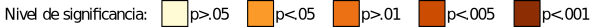
\includegraphics[scale=.7]{./img_art_dfa/escala.pdf} \\
\caption{Regiones donde la cantidad de ventanas estacionarias es significativamente diferente 
durante sueño MOR y NMOR, usando ventanas de 30 segundos}
\label{cabeza_new}
\end{figure}

Se repitió la comparación a un nivel grupal, usando la prueba $U$ de  Mann-Whitney.
Se encontraron diferencias significativas para el grupo CTL en los canales P3, P4, PZ, 
ROG y EMG; en el grupo PDC se observaron tales diferencias sólo en P4.
%
Las proporciones muestran tendencias que, quizá, resultaron no ser significativas
por el tamaño pequeño de la muestra: los canales P3 y PZ podrían ser diferentes también para
individuos del grupo PDC, y el canal LOG podría ser diferente durante sueño MOR y NMOR.
%
Así mismo se hipotetiza que para el grupo CTL, en todos los canales, el sueño MOR
es presenta menor cantidad de épocas estacionarias.

Se concluye que
no se puede establecer diferencias entre las medias grupales para esta cantidad (proporción de
épocas estacionarias, medidas en el sentido de PSR), debido a la gran variabilidad entre sujetos.

\begin{figure}
\centering
\includegraphics[width=\linewidth]
{./img_art_dfa/Comparacion_gpos_CTL_PDC_v3.pdf}
\caption{Proporciones de épocas estacionarias, durante sueño MOR y NMOR.}
\label{comparacion_verde}
\end{figure}

\begin{figure}
\centering
\includegraphics[width=\linewidth]
{./img_art_dfa/Comparacion_gpos_MOR_NMOR_v3.pdf}
\caption{Proporciones de épocas estacionarias, grupos CTL y PDC.}
\label{comparacion_graf}
\end{figure}

%%%%%%%%%%%%%%%%%%%%%%%%%%%%%%%%%%%%%%%%%%%%%%%%%%%%%%%%%%%%%%%%%%%%%%%%%%%%%%%%%%%%%%%%%%%%%%%%%%%
%%%%%%%%%%%%%%%%%%%%%%%%%%%%%%%%%%%%%%%%%%%%%%%%%%%%%%%%%%%%%%%%%%%%%%%%%%%%%%%%%%%%%%%%%%%%%%%%%%%
%%%%%%%%%%%%%%%%%%%%%%%%%%%%%%%%%%%%%%%%%%%%%%%%%%%%%%%%%%%%%%%%%%%%%%%%%%%%%%%%%%%%%%%%%%%%%%%%%%%

\chapter{Discusión y conclusiones}

Una práctica común en el análisis de señales electrofisiológicas es el suponer que una serie de 
tiempo \textit{suficientemente} corta pueda considerarse estacionaria, cuando menos en el sentido
débil; anteriormente se ha señalado que se trata de un efecto de muestras pequeñas \cite{Melard89},
y paralelamente se han incorporado a los diseños experimentales motivos para mantener este supuesto
\cite{Kaiser00}.

Este trabajo parte de la hipótesis de que adultos mayores con PDC presentan en mayor medida 
estacionariedad débil en sus registros de PSG; al comparar sujetos de los grupo Nn (control) y Mn 
(PDC), no se observaron cambios significativos en la porción de tiempo durante la cual el registro 
de PSG se comporta como débilmente estacionario. 
Esto puede interpretarse como que los cambios en la corteza cerebral durante el deterioro 
cognitivo, no provocan que  la señal se vuelva más \textit{simple} en el sentido de 
\textit{volverse} estacionaria.

Comparando grupalmente la cantidad de épocas estacionarias durante MOR y NMOR, se encontró que en 
el grupo Nn había diferencias significativas en sitios de la región frontal y que no eran presentes
en el grupo Mn; para poder establecer una relación con el PDC haría falta un mayor grupo muestral, 
o bien nuevos registros de PSG para los mismos sujetos, o incluso analizar registros de EEG durante 
otro tipo de actividades y confirmar las diferencias encontradas.

Cabe destacar que la evidencia aportada indica que el PSG es un conjunto de señales que se comportan
como no-estacionarias durante la mayor parte del sueño, lo cual confirma el supuesto usual de que 
las señales de origen biológico son por naturaleza no-estacionarias. 
%\subsection{Efecto del tamaño de las época}

%En el apéndice X se explica que si disminuye el tamaño de época el test de PSR disminuye su 
%potencia, de modo que es más propensa a dar falsos negativos (rechazar la hipótesis de 
%estacionariedad cuando debía aceptarse); entonces, en épocas más pequeñas debería haber más épocas 
%clasificadas como no-estacionarias.
%Sin embargo, al \textit{graficar} la estacionariedad para diferentes tamaños de época (figura
%\ref{comp_VCR}) ocurre que es más frecuente el efecto contrario.
%
%\begin{figure}
%\centering
%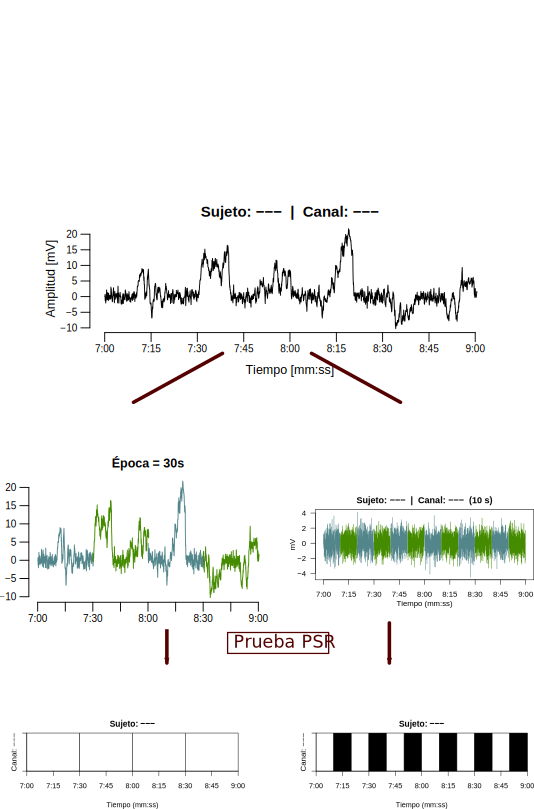
\includegraphics[width=\linewidth]{./img_diagramas/epocas_diferentes_v2.pdf}
%\caption{Efecto del tamaño de ventana sobre la clasificación de estacionariedad}
%\label{epocas_diferentes}
%\end{figure}
%
%Se propone que este efecto puede ser explicado si los registros de PSG son \textbf{localmente
%estacionarios}, una propiedad introducida por Dahlhaus \cite{Dahlhaus97} y que consiste en que un
%proceso no-estacionario pueda ser aproximado a trozos \textit{ensamblando} procesos estacionarios
%definidos para intervalos pequeños de tiempo.
%Esta caracterización del EEG ha sido usada anteriormente de manera fructífera pero problemática
%[??].
%
%En el contexto particular del presente trabajo, la presencia de estacionariedad local puede ser
%explicada fisiológicamente por el contenido heterogéneo de ritmos cerebrales de las etapas de 
%sueño; como ejemplo, en la etapa N3 aparecen husos de sueño mezcladas con ritmos Alfa, de modo
%que es posible hallar un fragmento de época en sueño N3 con únicamente un tren de ondas Alfa
%o un tren de husos de sueño.
%Este fenómeno es ilustrado de manera esquemática en la figura \ref{epocas_diferentes}.
%
%
%
%Entonces, se propone que los registros de PSG se comportan como procesos localmente estacionarios; 
%más aún, se propone que esta característica cambia cualitativamente en adultos mayores con PDC,
%para los cuales el \textit{nivel de homogeneidad} del PSG es muy similar durante MOR y NMOR.

%%%%%%%%%%%%%%%%%%%%%%%%%%%%%%%%%%%%%%%%%%%%%%%%%%%%%%%%%%%%%%%%%%%%%%%%%%%%%%%%%%%%%%%%%%%%%%%%%%%
%%%%%%%%%%%%%%%%%%%%%%%%%%%%%%%%%%%%%%%%%%%%%%%%%%%%%%%%%%%%%%%%%%%%%%%%%%%%%%%%%%%%%%%%%%%%%%%%%%%

\section{Conclusiones}

Se concluye que
es posible la ocurrencia de fragmentos arbitrariamente cortos de registros de PSG que no 
son débilmente estacionarios. Paralelamente, la presencia de estos fragmentos se ve influida por el
estado de actividad del cerebro.
%
Como consecuencia directa de este fenómeno, es posible limitar los efectos \textit{distorsivos} de 
la no-estacionariedad, para lo cual basta un diseño experimental que distinga adecuadamente el
estado de actividad a estudiar. 

En otro ámbito, es en principio posible usar la
proporción de estacionariedad (\textit{densidad} de ventanas estacionarias en el sentido de
PSR) en el EEG para caracterizar estados de actividad cerebral. Para ello, falta 
investigar las características particulares de la etapa que se busca identificar, así como otras
etapas cercanas en el tiempo.

%%%%%%%%%%%%%%%%%%%%%%%%%%%%%%%%%%%%%%%%%%%%%%%%%%%%%%%%%%%%%%%%%%%%%%%%%%%%%%%%%%%%%%%%%%%%%%%%%%%
%%%%%%%%%%%%%%%%%%%%%%%%%%%%%%%%%%%%%%%%%%%%%%%%%%%%%%%%%%%%%%%%%%%%%%%%%%%%%%%%%%%%%%%%%%%%%%%%%%%

\section{Trabajo a futuro}

Una vez que se ha identificado un marcador para el PDC usando un grupo de laboratorio,
conviene automatizar los análisis para su uso clínico sobre un público más general.
%
Un uso más amplio de la técnica asegura una mayor población para poder estudiar la 
efectividad y sensibilidad de la prueba
Y más que eso, se espera que puedan ser sinceramente beneficiosos para los pacientes. Siguiendo el
protocolo usual, los marcadores presentados no serán usados como único recurso para generar
un diagnóstico clínico, sino como un apoyo a las herramientas existentes.

El uso de marcadores basados en registros de PSG --basados en el EEG en general-- aporta una
base fisiológica al diagnóstico de deterioro cognitivo, misma que no es posible usando
únicamente pruebas neuropsicológicas.
%
Conviene destacar que, de entre las herramientas para el registro fisiológico del sistema nervioso
central, las técnicas electrofisiológicas son las más económicas y menos invasivas;
generar marcadores basados en ellas facilita su uso por el público general como herramienta 
diagnóstica, sobre todo en ausencia de síntomas.

%%%%%%%%%%%%%%%%%%%%%%%%%%%%%%%%%%%%%%%%%%%%%%%%%%%%%%%%%%%%%%%%%%%%%%%%%%%%%%%%%%%%%%%%%%%%%%%%%%%
%%%%%%%%%%%%%%%%%%%%%%%%%%%%%%%%%%%%%%%%%%%%%%%%%%%%%%%%%%%%%%%%%%%%%%%%%%%%%%%%%%%%%%%%%%%%%%%%%%%
%%%%%%%%%%%%%%%%%%%%%%%%%%%%%%%%%%%%%%%%%%%%%%%%%%%%%%%%%%%%%%%%%%%%%%%%%%%%%%%%%%%%%%%%%%%%%%%%%%%
